\subsection{Gameplay UI}
\label{sec:UI_Gameplay}
The main interaction UI used throughout \ourgame{} will be placed at the bottom of the screen and will present options to the player character in bubbles. These bubbles will be context sensitive. In Figure~\ref{fig:UI_npc_talk}, the player is looking at an NPC, so the bubbles include the options described in Section~\ref{sec:conversation}. Figure~\ref{fig:UI_npc_conversation} shows the UI during conversations. All of the UI representative of the player and their actions will be one hue, and all of the UI representative of other characters will be shown in a different hue.

\begin{figure}[htb]
  \centering\begin{subfigure}{.33\textwidth}
    \centering
    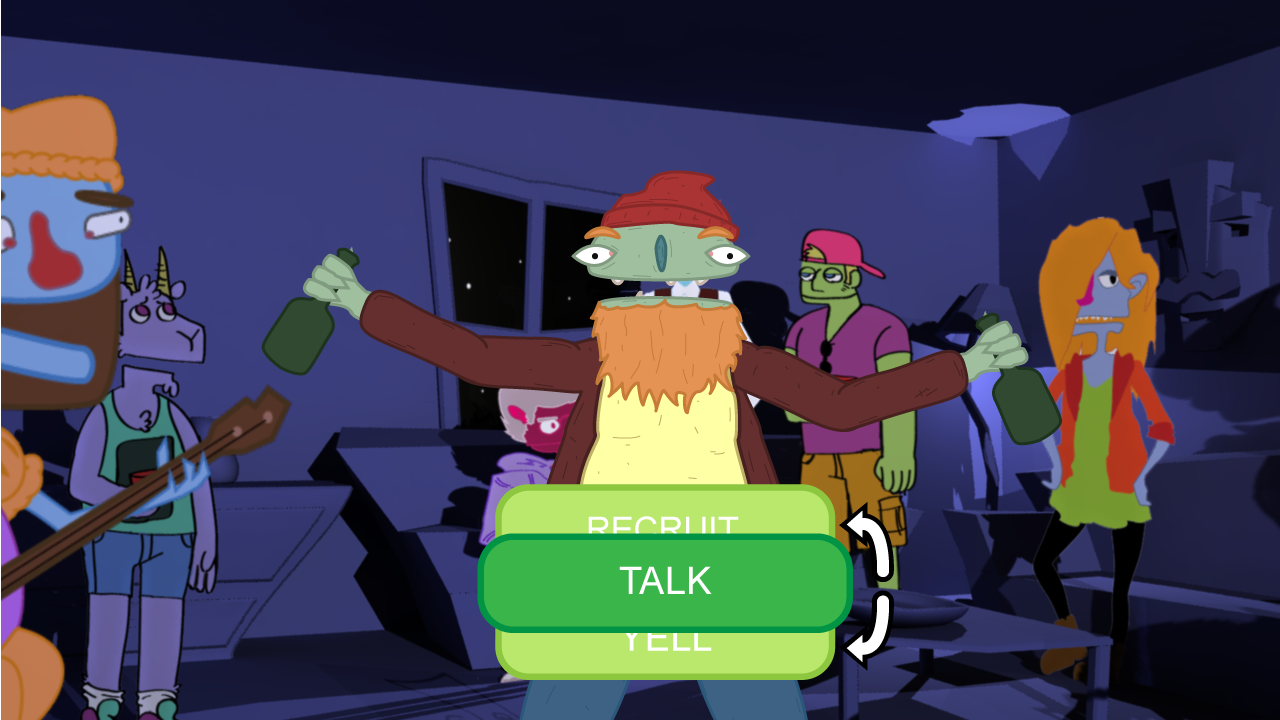
\includegraphics[width=.9\linewidth]{images/UI_npc_talk}
    \caption{NPC UI}
  	\label{fig:UI_npc_talk}
  \end{subfigure}%
  \begin{subfigure}{.33\textwidth}
    \centering
    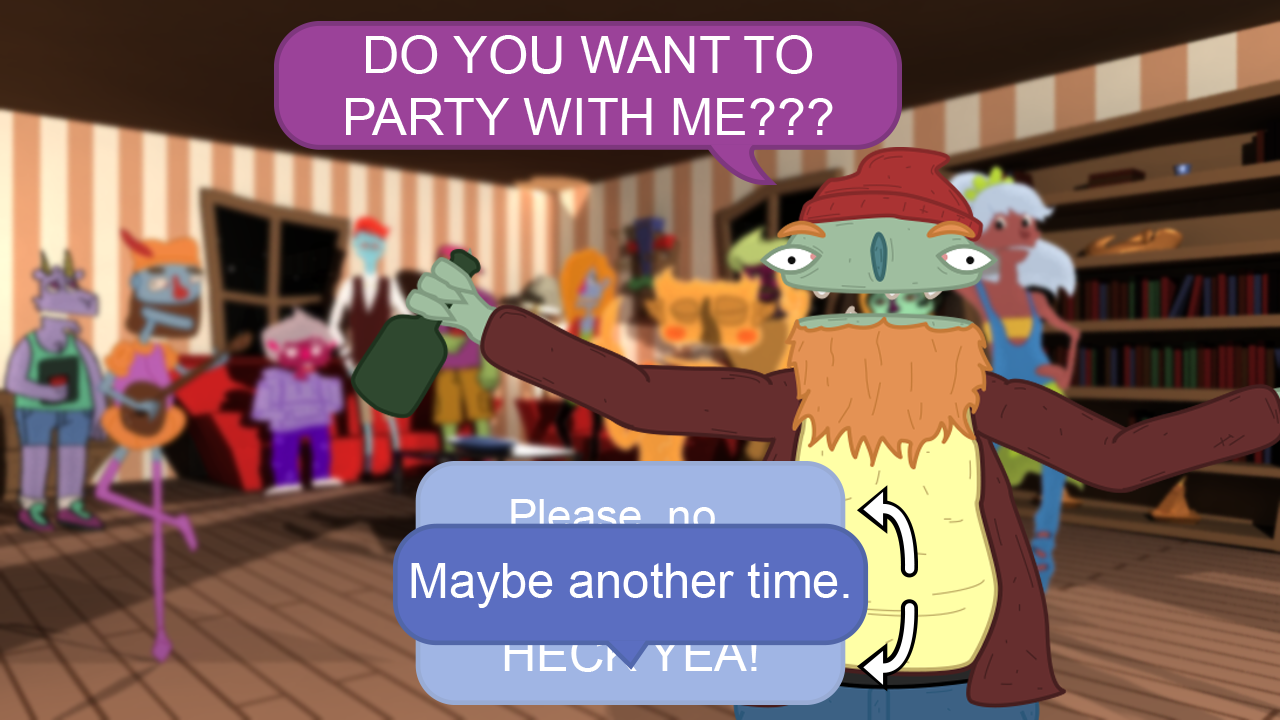
\includegraphics[width=.9\linewidth]{images/UI_npc_conversation}
    \caption{Conversation UI}
  	\label{fig:UI_npc_conversation}
  \end{subfigure}%
  \caption{Bubble interaction UI}
  \label{fig:gameplay_UI}
\end{figure}

The gameplay UI will also include a map and a task list. The map will be a grid showing visited rooms in the upper-right corner of the screen, and the task list will show a list of hints and progress messages in the upper-left corner of the screen. Occasionally, an additional message popup may be triggered in the center of the screen in order to present more contextual information to the user.